\section*{TCP: Tcpdump}
A tcpdump packet capture was started and the scan written to a WireShark compatible pcap file for analysis. The tcpdump terminal output is shown in Listing~\ref{list:tcp_tcpdump}. The Ncat terminal output where the group member's names and MAC ID numbers were echoed is shown below in Listing~\ref{list:echo}.

\begin{lstlisting}[caption=Tcpdump Packet Capture of Python Echo Server Connection,label=list:tcp_tcpdump]
sudo tcpdump -nnvvX -i 1 -S host compeng4dn4.mooo.com -w mooo_echo.pcap
tcpdump: listening on eth0, link-type EN10MB (Ethernet), snapshot length 262144 bytes
21 packets captured
88 packets received by filter
0 packets dropped by kernel
\end{lstlisting}

\begin{lstlisting}[caption=Ncat Connection to Python Echo Server,label=list:echo]
ncat --crlf compeng4dn4.mooo.com 50007
Wecome to COMPENG 4DN4 Echo Server!
Raeed Hassan
Raeed Hassan
400188200
400188200
Aaron Pinto
Aaron Pinto
400190637
400190637
\end{lstlisting}

The capture displayed in WireShark is shown below in Figure~\ref{fig:echo_wireshark}. The first three packets (1-3) contain the three way handshake which establishes the TCP connection. The next two packets are (4-5) shows that the server is letting the host know that it is sending some data in packet 4 (the message "Wecome to COMPENG 4DN4 Echo Server!") while acknowledging the last signal with a [PSH, ACK] signal, and that the host acknowledges this in packet 5. 

Packets 6-9 are for the first message sent to the server ("Raeed Hassan") which is echoed back to the host. The host sends the message in packet 6, with a [PSH, ACK] signal as discussed earlier, which is then acknowledged by the server in packet 7. The server then does the same when echoing the message back, with a [PSH, ACK] signal in packet 8, which is acknowledged by the host in packet 9. 

For the next three messages, the ACK signal from the server (such as in packet 7) is dropped and instead only 3 packets are sent, a [PSH, ACK] signal from the host to the server when sending the message, a [PSH, ACK] signal from the server to the host when it echoes back the signal, and an ACK signal from the host acknowledging the previous signal. Packets 10-12 are for the next message sent to the server ("400188200") which is echoed back to the host. Packets 13-15 are for the next message sent to the server ("Aaron Pinto") which is echoed back to the host. Packets 16-18 are for the next message sent to the server ("400190637") which is echoed back to the host. 

The last three packets (19-21) close the TCP connection. The host sending sends a FIN signal in packet 19 to indicate it wishes to finish the TCP connection, which the server acknowledges in packet 20 and sends back it's own FIN signal. The connection is finished as the host acknowledges the server's signal in packet 21.

\begin{figure}[htp]
\centering
\caption[echo_wireshark]{Tcpdump Capture of Python Echo Server in WireShark}\label{fig:echo_wireshark}
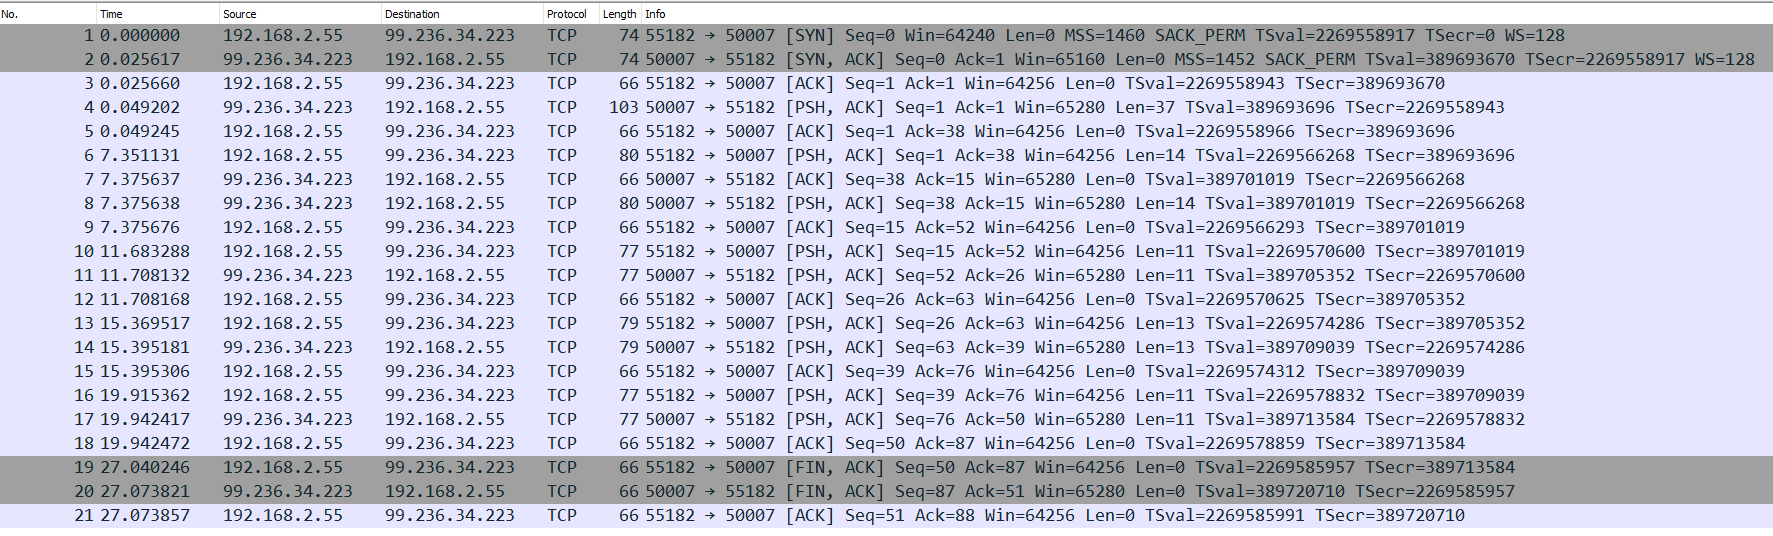
\includegraphics[width=\textwidth]{echo_server.png}
\end{figure}